\documentclass[12pt,letterpaper,oneside]{book}

\usepackage{afitStyleFiles/afitThesis}
\usepackage{afitStyleFiles/sf298}
\usepackage[acronym, toc,shortcuts]{glossaries}
\usepackage{algorithm}
\usepackage{algpseudocode}
\usepackage{bm}
\usepackage[table,xcdraw]{xcolor}
\usepackage{listings}
\usepackage{multirow}
\usepackage{physics}
\usepackage{rotating}
\usepackage{silence} \WarningFilter{fixltx2e}{}
\usepackage{stringstrings}
\usepackage{titlecaps}
\usepackage{cleveref} % for \Cref, etc.
\usepackage{textcomp}
\usepackage{siunitx} % for using scientific notation for numbers, can include units easily and "x10^6" etc.
\usepackage[section]{placeins}
\lstset{basicstyle=\ttfamily,breaklines=true}
\sisetup{
	round-mode          = places, % Rounds numbers
	round-precision     = 3, % to 2 places
	per-mode=symbol,
	% fraction-function=\sfrac % for different style of fractions
}

% KJ Nelson added to afitThesis.sty:
%\usepackage[hyphens]{url}
%\usepackage{hyperref}
\usepackage{minted}

\usepackage[final]{pdfpages}

\graphicspath{{Figures/}}
%% Customize your document with your personal information
%% First, comment out the appropriate document type
\afitthesis %%default
% \afitreport
% \dissertation
% \prospectus

\author{First M Last, B.S.E.E.}
\rank{Captain, USSF} % If a civilian, comment out this line.

\docdesignator{AFIT-ENG-MS-20-M-XXX} % Update from list from 
\department{Department of Electrical and Computer Engineering}
\graduationdate{March 19, 2022}

\flytitle{THESIS TITLE} 
\title{THESIS TITLE}
                             % Note, if you use \MakeUppercase to put
                             % the title in all uppercase as the style
                             % guide demands, understand that the
                             % command does not allow page breaks ``\\'' 
                             % within its brackets.
\previousdegrees{B.S.E.E.}
\acdegree{Master of Science in Electrical Engineering}

\committee{{First M Last,, Ph.D\\Chair},
           {First M Last,, Ph.D\\Member},
           {First M Last,, Ph.D\\Member}}

\address{2950 Hobson Way\\ Air Force Institute of Technology \\
Wright-Patterson AFB, OH 45433}

\distribution{DISTRIBUTION STATEMENT A\\[-10pt]
\MakeUppercase{Approved for Public Release; distribution unlimited.}
} 

\disclaimer{The views expressed in this document are those of the
author and do not reflect the official policy or position of the
United States Air Force, the United States Department of Defense or
the United States Government.  This material is declared a work of the
U.S. Government and is not subject to copyright protection in the
United States.}

% International students may consider using the following disclaimer
% statement: \dislaimer{The views expressed in this document are those
% of the author(s) and do not reflect the official policy or position
% of the United States Air Force, Department of Defense, United States
% Government, the corresponding agencies of any other government,
% NATO, or any other defense organization.}

	
%\makenoidxglossaries
\loadglsentries{myThesis/glossary}

\begin{document}
%\glossaryAcronyms
{\frontmatter
\flyleaf                        
\disclaimerpage                 
\titlepageAFIT                      
\committeepage  }
\phantomsection
\begin{abstract}	
	
Abstract text here. Put in acronyms, like \gls{UAV}. Or cite items like with \cite{Scaramuzza2011} in a bibtex file auto-updated from Mendeley.
	
\end{abstract}

\begin{dedication}
To my wife.  Without your love, companionship, and support, I would have never seen the completion of this work.

To my brothers of Theta Tau.  You all are, and always will be, my family.
\end{dedication}

\chapter*{Acknowledgments}
I would like to thank my advisor, ...



\phantomsection %not sure exactly what this does, but it helps with Table of Contents and References
{
\tableofcontents
\glsunsetall % resets all acronyms, so all will be spelled out again
%\listoffigures
%\listoftables
% UNUSED
%\listofabbreviations
%\listofsymbols
	
\mainmatter }
\phantomsection
\chapter{Introduction}
\label{ch:introduction}
\glsresetall

\section{Problem Background}

Text here

\subsection{Subsection Title Here}

Subsection text here


\section{Research Objectives}

Research objectives here.

\section{Document Overview}

Reference chapters, papers and sections like \cref{ch:introduction}.

\phantomsection
\chapter{Paper: Temporal Consistency}
\label{ch:temporal_consistency}

The following paper, ``Characterizing, Measuring, and Validating the Temporal Consistency of Live-Virtual-Constructive Environments,'' was submitted and accepted by the Society for Modeling and Simulation International (SCS); it was published in October of 2009.

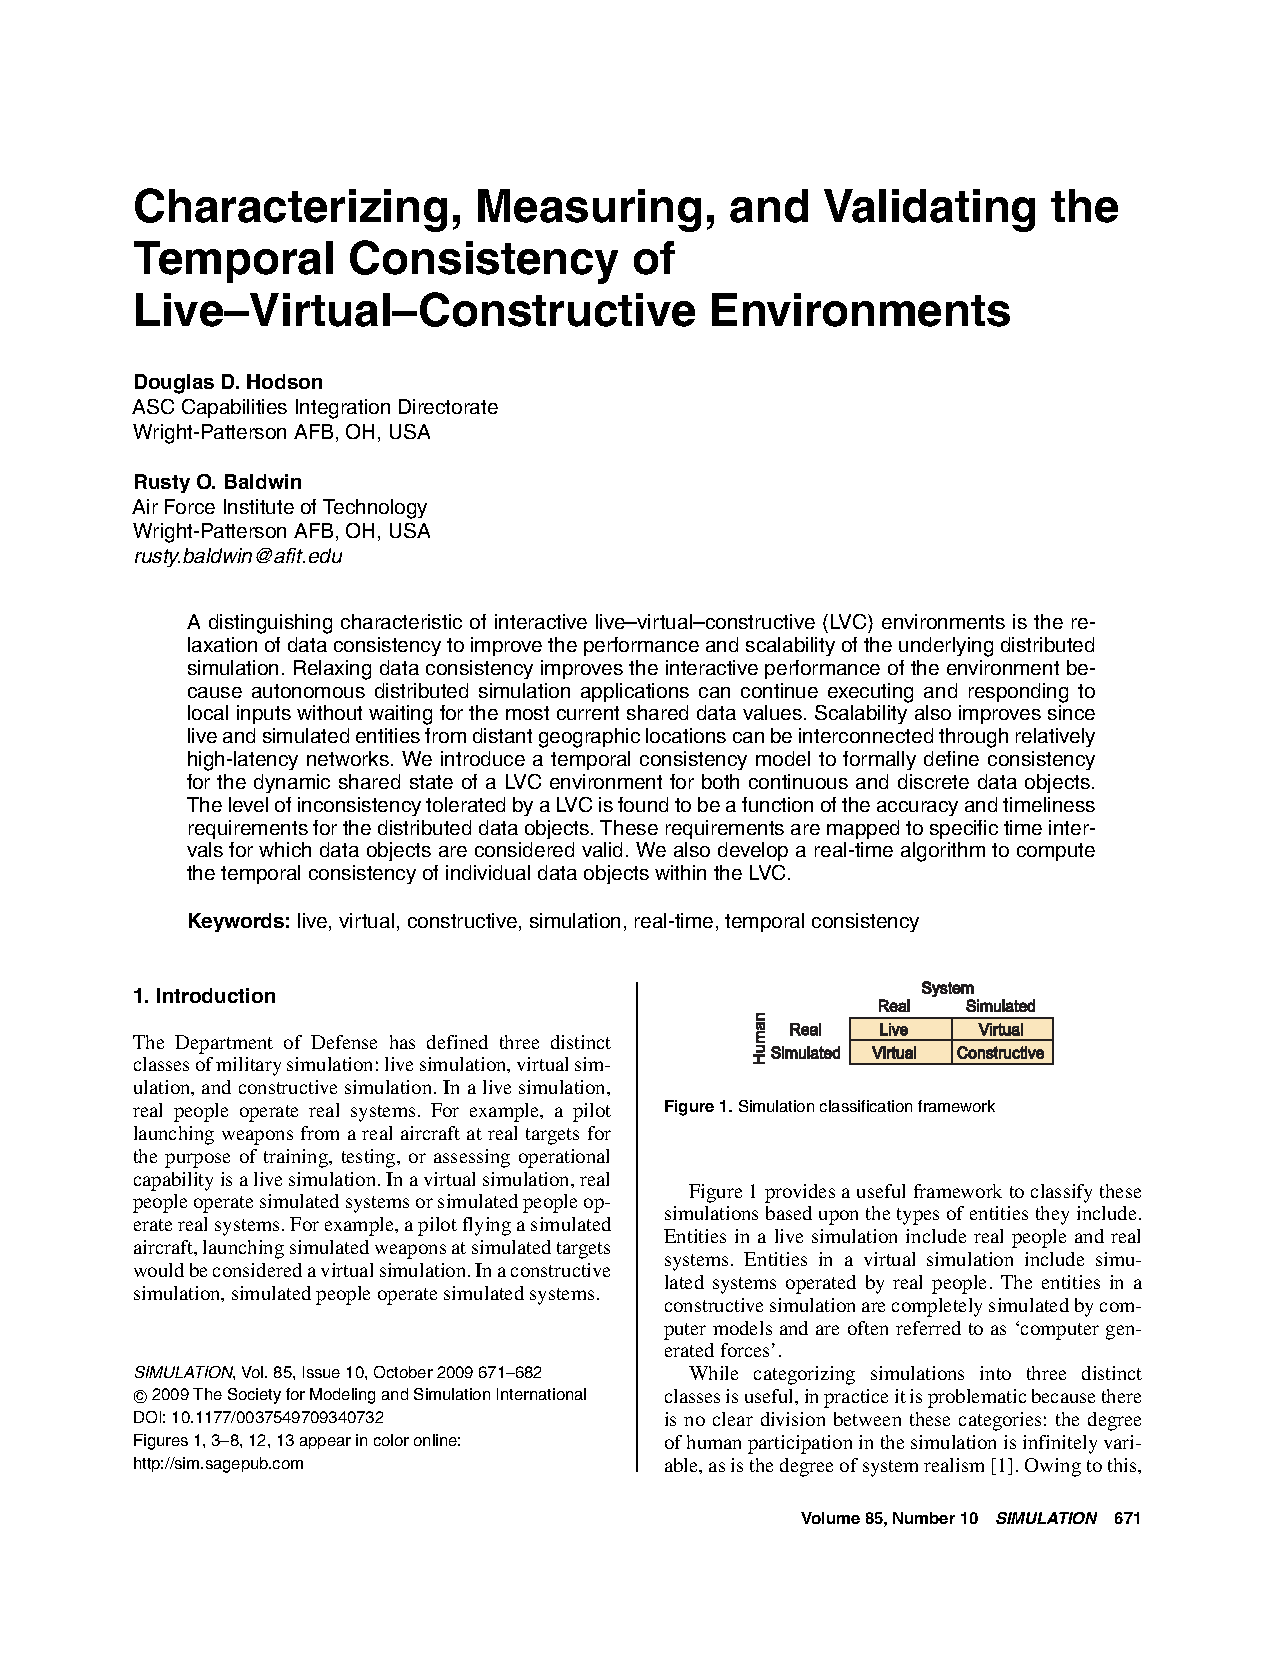
\includepdf[pages=-]{papers/v2009_10-scs-simulation-temporal-consistency}

\phantomsection
\chapter{Paper: Art and Science of LVC}
\label{ch:art_and_science}

The following paper, ``The Art and Science of Live, Virtual, and Constructive Simulation for Test and Analysis,'' was submitted and accepted by the Journal of Defense Modeling and Simulation (JDMS); it was published in April of 2014. 

\includepdf[pages=-]{papers/v2014_04-jdms-art-and-Science-of-lvc}

\phantomsection
\chapter{Conclusions}
\label{ch:conclusion}
\glsresetall
{
Conclusion text here.
}
\section{Future Work}
{
Text here

\begin{itemize} % bulleted list
	
	\item Item 1 text here.
	
	\item Item 2 text here.

\end{itemize}
}
\phantomsection
%%%%%%%%%%
% if Appendix is needed:
%%%%%%%%%%
\renewcommand{\theHchapter}{A\arabic{chapter}}
\appendix
%	\begin{appendices}
\phantomsection

\chapter{Additional Results}
\label{app:addResults}

%More Results Figures here, if desired.

\chapter{Second Appendix Title}
%
%e.g. include significant MATLAB Code


\phantomsection
%\input{myThesis/library.tex}
\bibliographystyle{IEEEtran}
%\bibliography{myThesis/myBibliography}
\bibliography{myThesis/library}
\phantomsection
%\printnoidxglossary[sort=word,type=acronym]
%\printglossary[type=abbrev]

\backmatter
\date{March 2020}
\ReportDate{19--03--2020} \ReportType{Master's Thesis}
\DatesCovered{Sept 2018 --- Mar 2020}

\Title{\centering {Thesis Title}\\
                  {with a Second Line}}

%\ContractNumber{DACA99--99--C--9999}

%\GrantNumber{}
%\ProgramElementNumber{}
%\ProjectNumber{09ENP???}
%\TaskNumber{}
%\WorkUnitNumber{}

\Author{First M. Last}

\PerformingOrg{Air Force Institute of Technology\\[-1pt]
    Graduate School of Engineering and Management (AFIT/EN)\\[-1pt]
    2950 Hobson Way\\[-1pt]
    WPAFB OH 45433-7765}

\POReportNumber{AFIT-ENG-MS-20-M-XXX} % Update with member-specific number

\SponsoringAgency{ AFXX/XXXX\\[-1pt]
Building XXX\\[-1pt]
WPAFB OH 45433-7765\\[-1pt]
DSN XXX-XXXX, COMM 937-XXX-XXXX\\[-1pt]
Email: first.last@us.af.mil }

\Acronyms{XXXX/XXXX}
%\SMReportNumber{}
\DistributionStatement{DISTRIBUTION STATEMENT A:\\[-1pt]
\MakeUppercase{Approved for Public Release; distribution unlimited.}}

\Abstract{Short abstract paragraph text here.}

\SubjectTerms{subject terms here}

\NumberPages{XXX} % update with exact number of pages for entire doc, including SF298, when complete
%\ReportClassification{}
%\PageClassification{}
%\AbstractClassification{}
\AbstractLimitation{UU}

\ResponsiblePerson{Captain First M. Last, AFIT/ENG}

\RPTelephone{(937) 255-3636, ext XXXX; first.last@afit.edu}

\MakeRptDocPage



\end{document}